\documentclass[12pt]{article}
\usepackage{amsmath}
\usepackage{graphicx}
\usepackage{float}

\usepackage{epsfig}
\usepackage{graphicx}
\usepackage{amsmath}
\usepackage{amsfonts}
\usepackage{amssymb}
\usepackage{amsthm}
\usepackage{longtable}
\usepackage[bf,labelsep=period,textfont=bf,justification=justified,singlelinecheck=false]{caption}
\usepackage[normalem]{ulem}
\usepackage{datatool}
\usepackage[nonumberlist,section=paragraph]{glossaries}
\usepackage{listings}
\usepackage{xcolor}
\usepackage{float}
\usepackage[version=4]{mhchem}
\usepackage{caption}
\usepackage{subcaption}
\usepackage{multicol}
\usepackage[absolute,overlay]{textpos}
\usepackage[export]{adjustbox}
\setlength\columnsep{30pt}

\usepackage[utf8]{inputenc}
\usepackage[english]{babel}

\newtheorem{theorem}{Theorem}

\title{Analytic Tools for the Finite Element Method on Parabolic Equations} 

\author{Geneva Porter, SDSU Spring 2020\\ 
Numerical Partial Differential Equations\\
Dr. Uduak George, Applied Mathematics}

\date{7 May, 2020} 
\begin{document}
\maketitle

The finite element method (FEM) is a technique used to solve many different types of partial differential equations on a variety of meshes. Almost always implemented numerically, the FEM has several practical applications in applied mathematics. This report will detail one particular application, solving a parabolic reaction-diffusion equation on a surface geometry, and discuss ways in which the theoretical application is valid. Then, we will compare the analytic solution on the surface of a sphere with a solution using the FEM. The proceeding error analysis will examine to solution L2 and H1 norms, as well as the difference when mesh density changes.

\section{The Finite Element Method}

Notes to add to thesis: add details from short explanation on FEM from "Stability, consistency, and convergence" by D Arnold.

\section{IMEX Scheme}

\section{Well-Posedness}

We can define a well-posed problem as having three characteristics:

\begin{enumerate}
	\item A solution for the problem exists
	\item The solution is unique
	\item The solution changes continuously as the boundary values and initial conditions change.
\end{enumerate}

To verify that the Schnakenberg system meets these requirements, recall the given equations with their boundary conditions and initial values using the variables $t$, $\phi$, and $\theta$:

\begin{equation}
	\begin{aligned}
		\dot{u} - \Delta_\Gamma u = \gamma f(u,v) ~~~~~ f(u,v) = \alpha - u + u^2v ~~~\\
		\dot{v} - \delta\Delta_\Gamma v = \gamma g(u, v) ~~~~~ g(u, v) = \beta - u^2v ~~~ \text{with}\\
		u(t,\pi, \theta) = u(t, -\pi, \theta) ~~~~~ u(t, \phi, \pi) = u(t, \phi, -\pi) \\
		v(t,\pi, \theta) = v(t, -\pi, \theta) ~~~~~ v(t, \phi, \pi) = v(t, \phi, -\pi)	\\
		\text{and} ~~~~~ u_0 = \alpha + \beta ~~~~~ v_0 = \frac{\beta}{(\alpha+\beta)^2}~~~~~~
	\end{aligned}
\end{equation}

This system is a parabolic reaction-diffusion system, which is guaranteed to be well-posed so long as there are at least 2 boundary conditions and the spatial derivative is of the second degree. We can see that there are indeed two boundary conditions and that the spatial derivatives $\Delta_\Gamma u$ and $\Delta_\Gamma v$ are of the second degree. We know the system is parabolic because it follows the form:

\begin{equation}
	\begin{aligned}
		A_1u_{xx} + 2B_1u_{xt} + C_1u_{tt} + D_1u_x + E_1u_t + F_1 = 0 \\
		A_2v_{xx} + 2B_2v_{xt} + C_2v_{tt} + D_2v_x + E_2v_t + F_2 = 0
	\end{aligned}
\end{equation}

Here, the spatial derivatives $\Delta_\Gamma u$ and $\Delta_\Gamma u$ are represented by $u_{xx}$ and $v_{xx}$, respectively. The time derivatives $\dot{u}$ and $\dot{v}$ are likewise represented by $u_t$ and $v_t$. For both equations, the coefficients corresponding to $B$ and $C$ are equal to zero, so the criteria for parabolic classification $B^2-AC=0$ is met.


\section{Consistency}

For FDM, consistency occurs when mesh cells and time step size decrease, the truncation error approaches zero. In other words, the discrete system should be a ``good" approximation of the partial differential equation system. Normally we would determine consistency by showing:

\begin{equation}
	P\phi - P_{k,h}\phi \rightarrow 0 ~~~\text{as} ~~~ k,~h \rightarrow 0
\end{equation}

However, for nonlinear PDEs, we need a different definition. Applying the FEM to the idea  of consistency changes some strategies as well.

One way to measure consistency is by examining the local truncation error. Recall the linear system we set up using the FEM-IMEX scheme:

\begin{equation}
	Ax=b
\end{equation}

To find the truncation error, we apply a simple check after solving the system:

\begin{equation}
	\text{local error} = ||b-Ax|| ~~~ \text{with} ~~~ ||.|| = \sqrt{\sum_i (b-Ax)_i^2}
\end{equation}

The truncation error is already an integral part of the algorithm for solving the linear system (in this case, the conjugate gradient method). We can apply a constraint that forces the solver to continue enumerating until the solution gives a truncation error below the desired amount. This feature also allows us to easily control the accuracy to order $r$, so long as we constrain the truncation error as being less than both $\mathcal{O}(k^r)$ and $\mathcal{O}(h^r)$ where $k$ is the timestep and $h$ is the diameter of each cell. We define order $r$ by the following inequality:

\begin{equation}
	||b-Ax|| \lessapprox h^{r_1}+k^{r_2}
\end{equation}

We can then say that the numerical scheme is consistent if it is accurate of order $r=(r_1,r_2)>0$.

We can now show that we achieved consistency, with of accuracy order (2,2), by graphically examining a few items of data collected when solving on the lung mesh. For changing the diameter of each cell, we simply scaled the entire mesh, rather than subdividing or eliminating cells. This was largely because the irregularity of the mesh does not allow refinement along curved manifolds; therefore, subdividing the mesh would not add detail to the figure. Likewise, increasing the cell diameters of the mesh without enlarging the figure would mean losing key element needed to analyze the lung. The following sections detail the...DO ON SPHERE OR LUNG?

\begin{enumerate}
	\item Plotting the local error vs. each time step for $t<10$ for various $k$, repeat plot for various $h$
	\item Plotting local error at steady state for $t=10$ vs. $k$ for various $h$
	\item Creating a table showing the elements that ensure accuracy of order 2.
\end{enumerate}

\section{Convergence}

While consistency examines the discretization of a system, convergence implies that the $solution$ to the discrete system is a ``good" approximation to the $solution$ of the partial differential equation system. Now, we cannot measure convergence in the traditional way, because it requires knowledge of the exact solution. The exact solution to the Schnakenberg system on the surface of a spherical domain in unknown. However, we can create a facsimile of the exact solution by producing an output using the smallest time step and cell size that is computationally feasible. 

If we call this exact solution facsimile $W_E$ while our approximate solution is $W_h$, then we can say that the solution converges given that the following criteria is satisfied:

\begin{equation}
	||W_h - W_E|| \lessapprox h^{q_1} + k^{q_2}
\end{equation}

So long as $q=(q_1,q_2) > 0$, the solution converges at rate $q$. Like consistency, we can also show this graphically with the following visualizations:

\begin{enumerate}
	\item Plotting the difference norm vs. time for various time step solutions at the same cell size
	\item plotting the difference norm vs. time for various cell sizes at the same time step
	\item plotting the difference norm at t=10 vs. timestep size for various cell sizes
\end{enumerate}


\section{Stability}

Stability in a finite difference system demands that the solution is persistent, that is, small perturbations or errors (such as round-off errors) in the data disappear over time. In addition, it implies that a change of the initial and boundary data leads to a comparable change in the numerical solution. This concept is identical for the finite element method. In fact, the formal definition tells us that our solution $must$ be stable, since it is consistent and converges \cite{Tadmor2012}:

\begin{theorem}
	Let $W_h$ be the solution of a numerical method consistent with a well-posed time-dependent problem; in particular, assume that it is accurate of order $r>0$. Then, if the numerical method is stable, its solution converges with $r$th-order convergence rate,
	$$||W_h - W|| \lessapprox \sum_{m=0}^n k\cdot ||\text{local error}|| \lessapprox h^{r_1} + k^{r_2}, ~~~t^n\in[0,T].$$
\end{theorem}



%The fundamental meta-theorem of numerical analysis implies that a discretization which is consistent and stable is also convergent \cite{Arnold2009}.

%One consequence of well-posedness is stability. The discretization of the PDE system is stable if the discrete problem is well-posed \cite{Arnold2009}. We can show stability graphically by observing the steady state solution, via plotting the L$_2$ norm. The norm is given by:






\pagebreak


\section{Error Analysis???}

\subsection{Mesh Refinement and Convergence}

For mesh refined 4 times: 1,536 active cells, 6,146 degrees of freedom, 0.139239 max diameter.

For mesh refined 5 times: 6,144 active cells, 24,578 degrees of freedom, 0.0697337 max diameter.

To examine how the choice of a mesh domain influences the convergence of the system, we examined 4 separate spherical surfaces of varying density. The sphere with the lowest density contained 96 quadrilateral cells on a spherical surface of unit-less radius 1. The next contained 384 cells, then 1,536, and finally 6,144. Note that each mesh was refined by a factor of 4, as each quadrilateral cell was sub-divided into 4 smaller cells with approximately half of their starting width. In this context, "width" is defined as the longest distance between two vertices n a single cell, and for these meshes, width always refers to the longest diagonal of the quadrilateral. 

After computing both the numeric solution using the FEM and the approximate analytic solution, we have a basis for testing our analysis. First, we can examine the convergence behavior for the four spheres from the numeric and analytic solutions. Figure \ref{fig:inner_norms} shows the convergence measure norms for $u$, given by:

$$ ||u||_C = \sqrt{\sum_n (u_{n} - u_{n+1})^2} $$

This measure is useful because it informs us about the behavior of the system over time. When the difference between terms becomes constant, we know that the system has reached an oscillatory steady state. Such behavior is typical for reaction-diffusion problems, particularly those with biochemical applications. 

\begin{figure}[H]
	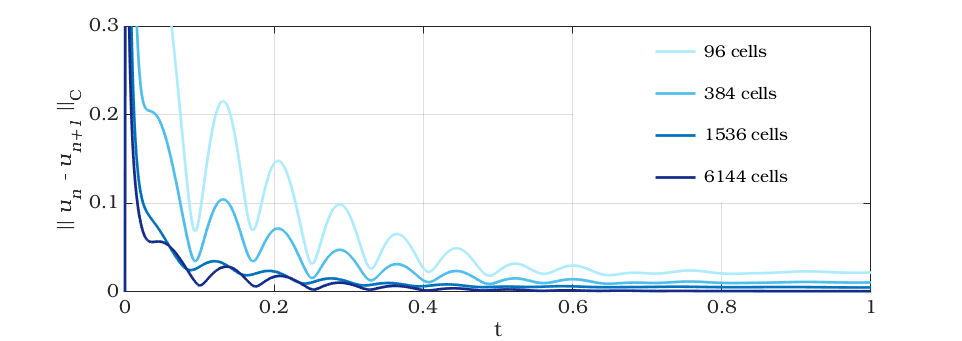
\includegraphics[width=\linewidth, trim= 1.4cm 0 2cm 0, clip]{norm_numeric.png}
	\caption{The L$_2$convergence measure norms for the numeric solution of the Schnakenberg system on a sphere.}
	\label{fig:inner_norms}
\end{figure}

Notice Figure \ref{fig:inner_norms} shows that for the numeric solutions, higher mesh density equates to a more stable convergence measure. In fact, as the width of the cells on the mesh halves, the value of the norm equilibrium halves as well. This is consistent with our previous findings, specifically Equation \ref{eq:error_cells}.

\section{Conclusion}

\end{document}






recall the linear system and it's boundary and initial data as discussed in section \ref{sec:analytic}:

\begin{equation}\label{eq:data}
\begin{aligned}
\text{For } W(t, \phi, \theta): ~& \dot{W} - \left(\begin{matrix} 
1 & 0 \\ 0 & \delta
\end{matrix}\right)\Delta_\Gamma W = \gamma~F ~~~ \text{with} ~~~ F = \left(\begin{matrix} 
\alpha - u + u^2v \\ \beta - u^2v
\end{matrix}\right) \\
~& W(t,\pi,\theta) = W(t,-\pi,\theta), ~~~ W(t,\phi,\pi) = W(t,\phi,-\pi)\\
~& W(0,\phi,\theta) = W_0 = 
\left(\begin{matrix} 
u^* \\ v^* 
\end{matrix}\right) = 
\left(\begin{matrix} 
\alpha + \beta \\ \frac{\beta}{(\alpha + \beta)^2} 
\end{matrix}\right)\\
~& W = 
\left(\begin{matrix} 
0 \\ 0 
\end{matrix}\right) ~~~ \text{on} ~~~ \partial\Gamma
\end{aligned}
\end{equation}






